% !TeX root = ../thuthesis-example.tex

\chapter{基于最优控制理论的触摸运动模型}

最优控制理论是数学最优化的分支,研究使动力控制系统的性能指标实现最优化的综合方法。自1962年Potryagin等人提出最优控制理论以来[xx],该理论被广泛应用于空间技术[]、电力系统控制[]、经济调控[]等重要领域。1985年,Tamar等人指出,最优控制理论还可用于描述人的手部运动过程[xx]。论文指出,人在手部运动的控制过程中,大脑并不会具体地控制肩关节和肘关节的旋转角度,而是将注意力集中在手部(由手掌和手指构成的整体),试图“\emph{在规定时间$t_1$内,最平稳地将手部从初始点$(x_0, y_0, z_0)$移动到目标点$(x_f, y_f, z_f)$}”。其中,“最平稳地”指的是人下意识地最小化手了部运动急动度平方的积分:

\begin{equation}
	C=\frac{1}{2}\int_{0}^{t_1}\left(\left(\frac{d^3x}{dt^3}\right)^2+\left(\frac{d^3y}{dt^3}\right)^2+\left(\frac{d^3z}{dt^3}\right)^2\right)dt
	\label{equ:objective_function}
\end{equation}

其中,$x(t)$,$y(t)$和$z(t)$是手部位置随时间变化的函数。受到这份工作的启发,本文作者通过实验验证发现,触摸运动过程同样可由公式\ref{equ:objective_function}描述。在此公式的约束下,本文提出了基于最优控制理论的触摸运动模型。本章分三部分介绍触摸运动模型:(1)触摸运动的数学模型,即描述触摸运动过程的数学方程;(2)触摸运动的计算模型,即利用运动传感信号(位移、速度、加速度时间序列)拟合触摸运动方程的最优化方法;(3)模型对触摸交互技术的指导性意义,即探讨触摸运动方程能给触摸交互技术带来哪些有用的信息,及如何利用这些信息改进交互技术。

\section{触摸运动的数学模型}

触摸运动的数学模型是描述触摸事件前后短暂时间内手指运动过程的数学方程。触摸运动的过程可描述为:“\emph{如图\ref{fig:touch_model_virtual}所示,若交互表面凭空消失,人会在时间$t_1$内最平稳地将手指从初始点$x_0$移动到目标点$x_1$。但实际情况是如图\ref{fig:touch_model_real}所示的情况,交互表面真实存在,手指会在时间点$t_c$因与交互表面接触而停止。}”,触摸运动的方程是:

\begin{figure}
	\centering
	\begin{subfigure}[b]{0.45\textwidth}
		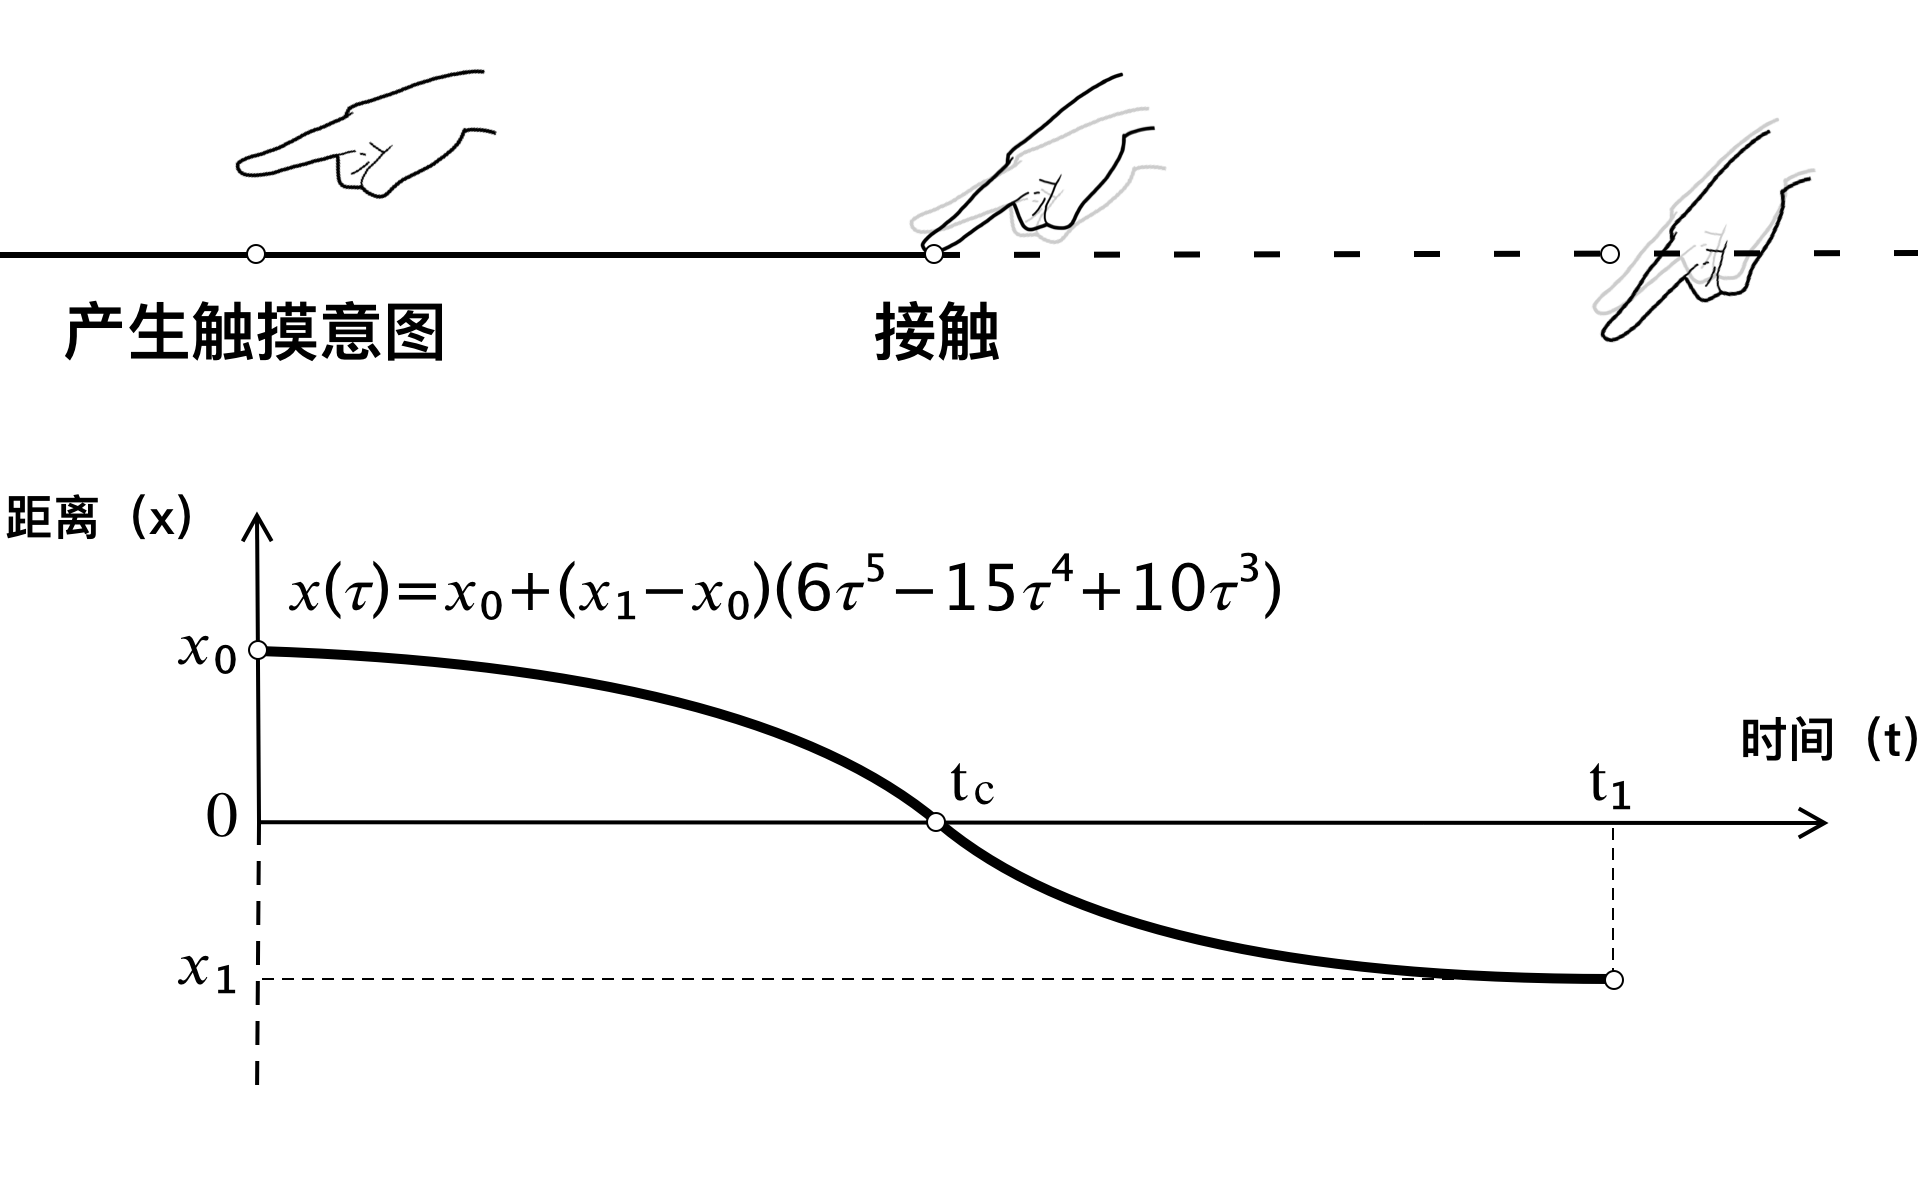
\includegraphics[width=\textwidth]{touch_model_virtual.png}
		\caption{若交互表面凭空消失}
		\label{fig:touch_model_virtual}
	\end{subfigure}\hfill% or \hspace{5mm} or \hspace{0.3\textwidth}
	\begin{subfigure}[b]{0.45\textwidth}
		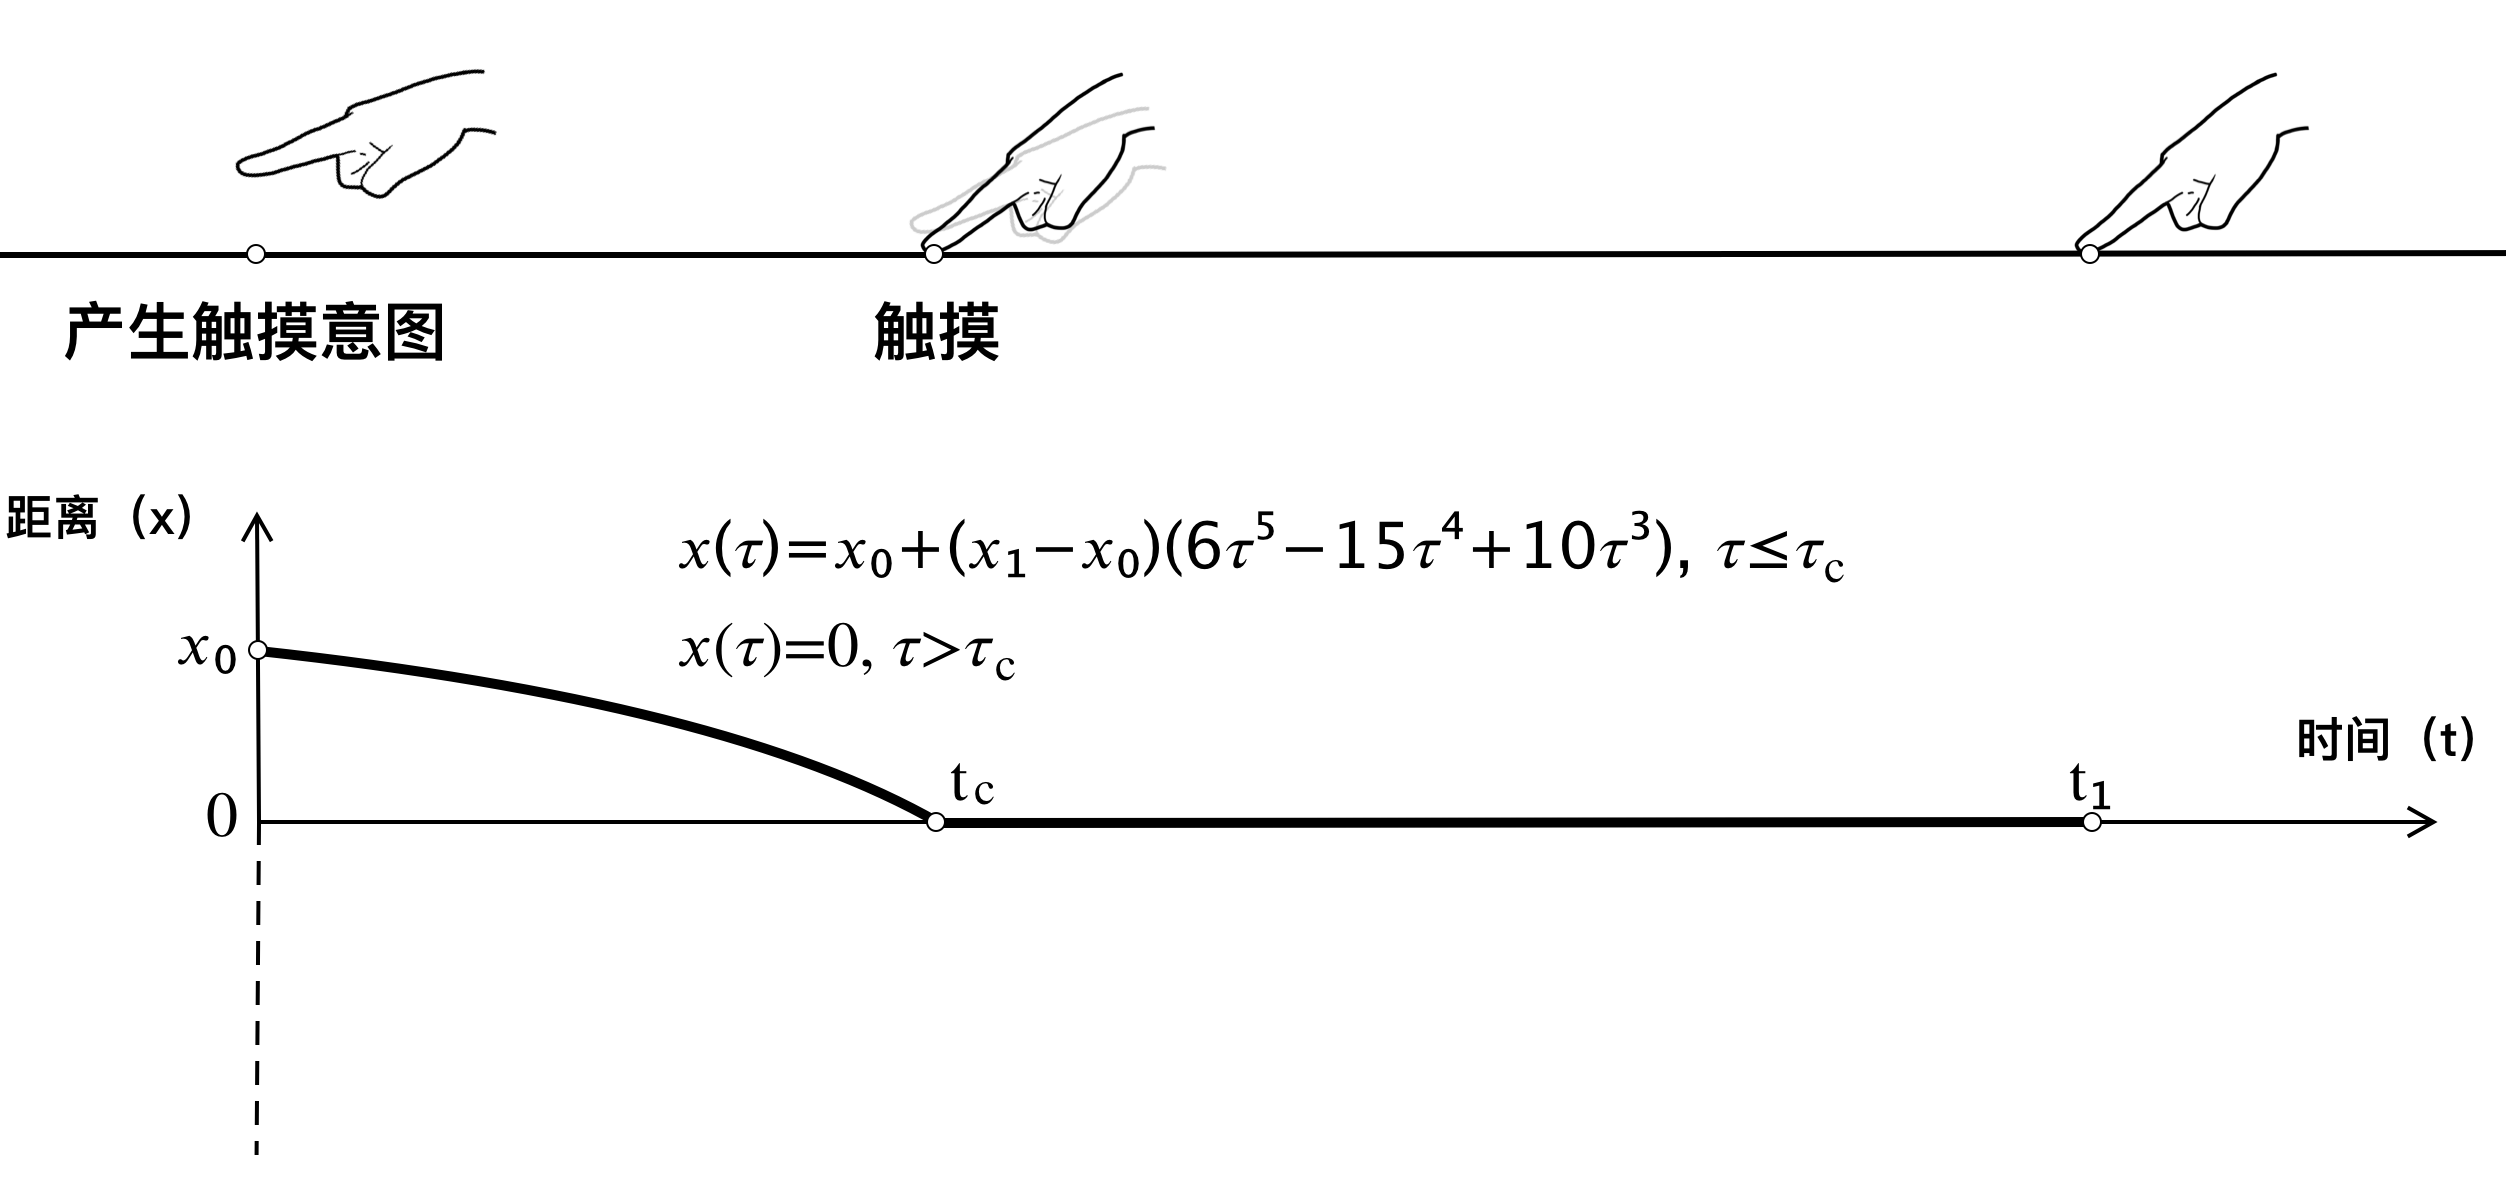
\includegraphics[width=\textwidth]{touch_model_real.png}
		\caption{实际情况}
		\label{fig:touch_model_real}
	\end{subfigure}
	\caption{基于最佳控制理论的触摸运动模型图示}
	\label{fig:touch_model}
\end{figure}

\begin{equation}
	x(\tau)=
	\begin{cases}
		x_0+(x_1-x_0)(6\tau^5-15\tau^4+10\tau^3)& \tau<=\tau_c \\
		0& \tau>\tau_c
	\end{cases}
\label{equ:touch_model}
\end{equation}

其中,$x$是手指与交互表面的高度之差,$\tau=\frac{t}{t1}$是时间进度。通过对上述函数的求导不难发现,触摸运动模型同时揭示了手指速度$v$和加速度$a$与时间$t$之间的关系:

\begin{equation}
v(\tau)=
\begin{cases}
	(x_1-x_0)(30\tau^4-60\tau^3+30\tau^2)& \tau<\tau_c \\
	0& \tau>\tau_c
\end{cases}
\end{equation}

\begin{equation}
	a(\tau)=
	\begin{cases}
		(x_1-x_0)(120\tau^3-180\tau^2+60\tau)& \tau<\tau_c \\
		0& \tau>\tau_c
	\end{cases}
\label{equ:touch_model_a}
\end{equation}

公式\ref{equ:touch_model}即为触摸运动的数学模型,本小节剩余内容将介绍模型的提出和推导过程。需要声明的是,本文提出的触摸运动模型是对触摸运动过程的良好拟合,后续章节会通过用户实验验证模型的预测精度。然而,同人机交互中许多经典的模型一样(如费茨定理[xx]),本模型的正确性是无法从人体机理的角度证明的,模型有可能在未来工作中会得到修正和完善。

本文中,触摸运动模型的提出源于一个非正式实验。如图xx所示,16名被试参与了实验,被试用食指连续地点击一块木板,实验者使用300Hz的高速摄像头记录被试手指的运动过程。在被试连续点击数次之后,实验者要求被试闭上双眼,继续点击。实验者在数秒后迅速移开木板,这一次,被试的手指触摸运动会“踏空”,实验也随即结束。每名用户只会进行一次实验,采集一次手指踏空的数据,而不会重复实验,这是为了防止用户知道实验意图之后,其触摸心理发生改变。高速摄像头记录的数据显示,在被试手指踏空的触摸运动中,其手指移动到了位于原来木板表面的高度之下,约1到3厘米的位置上。实验表明,人在组织一次触摸时,其心理并非将手指从初始点带到交互表面上,而是将手指带到交互表面之下的一个虚构点上。

【图:手指踏空实验】

根据最优控制理论,用户组织触摸运动的心理可描述为:“在规定时间$t_1$内,最平稳地将手部从初始点$(x_0, y_0, z_0)$移动到目标点$(x_1, y_1, z_1)$。”其中,“最平稳地”指的是最小化手指运动急动度的平方的积分(公式\ref{equ:objective_function})。为了简化触摸运动方程,作者假设手指在触摸运动的初始点和目标点上都是静止的,即速度和加速度同时为零。该假设是近似的,是考虑到当前传感器精度有限而做出的折中的约束条件,这是因为,如果运动方程的约束条件太少,运动方程的未知变量会变多,使得实际工程项目中很难以有限的运动传感精度和采样率拟合出准确的触摸运动轨迹。综上所述,若交互表面凭空消失,求解触摸运动方程等价于以下最优化问题:

\begin{equation}
	\begin{cases}
		x(t),y(t),z(t) \\
		s.t. x(0)=x_0,x^{'}(0)=x^{''}(0)=0,x(t_1)=x_1,x^{'}(t_1)=x^{''}(t_1)=0 \\
		y(0)=y_0,y^{'}(0)=y^{''}(0)=0,y(t_1)=y_1,y^{'}(t_1)=y^{''}(t_1)=0 \\
		z(0)=x_0,z^{'}(0)=x^{''}(0)=0,z(t_1)=z_1,z^{'}(t_1)=z^{''}(t_1)=0 \\
		min\frac{1}{2}\int_{0}^{t_1}\left(\left(\frac{d^3x}{dt^3}\right)^2+\left(\frac{d^3y}{dt^3}\right)^2+\left(\frac{d^3z}{dt^3}\right)^2\right)dt
	\end{cases}
\end{equation}

读者可能注意到,手部运动应该受到人的运动能力的限制,比如手部运动存在一个速度或加速度的上限。然而,上述最优化问题未包含对运动能力作出条件约束,这是因为,该问题的解天然地不会产生超出手部运动能力限制的情况[xx]。作者将上述最优化问题的求解过程写在附录xx中,此处直接给出问题的解:

\begin{equation}
	\begin{cases}
		x(\tau)=x_0+(x_1-x_0)(6\tau^5-15\tau^4+10\tau^3) \\
		y(\tau)=y_0+(y_1-y_0)(6\tau^5-15\tau^4+10\tau^3) \\
		z(\tau)=z_0+(z_1-z_0)(6\tau^5-15\tau^4+10\tau^3)
	\end{cases}
\end{equation}

上述公式表明,在触摸运动方程中,手指在$x$、$y$、$z$三个轴上的时空运动轨迹是相互独立的。本文在选题背景中已经阐述,本文的研究重点在于提高触摸交互的普适性、响应性和有意性,而不关心触摸在交互表面上2D位置的识别,因此,我们仅保留上述公式中$x$轴上的时空轨迹函数,作为触摸运动模型的表述(公式\ref{equ:touch_model})。

\section{触摸运动的计算模型}

触摸运动的计算模型是在已知数学模型的情况下,利用位移、速度、加速度等传感器信号来拟合触摸运动方程参数的计算方法。在工程技术中,常见的运动信号传感方法主要有(1)基于视觉方法的位移传感,和(2)基于运动传感器的加速度传感。由于速度传感器大多通过位移除以时间来计算,本文只讨论位移信号,而省去速度信号。

实验观察发现,一次触摸运动从用户产生触摸意图(手指开始加速运动),到手指触碰到交互表面的时长最短不低于50毫秒,最长不超过200毫秒。因此,从实用的角度出发,触摸运动的计算模型应该讨论,如何利用触摸事件发生前50毫秒的采样数据拟合触摸运动方程。假设我们用采样频率为$f_x$的位移传感器和采样频率为$f_a$的加速度传感器监测手指运动,在触摸发生前50毫秒内收集到以下数据:

\begin{equation}
\begin{cases}
[X_1, X_2, \cdots, X_n]& n=\lfloor0.05f_x\rfloor \\
[A_1, A_2, \cdots, A_m]& m=\lfloor0.05f_a\rfloor
\end{cases}
\end{equation}

则触摸运动的计算模型是利用上述时间序列拟合触摸运动方程(公式\ref{equ:touch_model})的计算方法。本小节剩余内容将按照计算顺序介绍此问题的解决方法。

\subsection{卡尔曼滤波}

卡尔曼滤波可用于控制测量数据的误触。研究工作中一般认为,基于视觉方法的位移信号和基于运动传感器的加速度信号的传感误差都符合正态分布[xx],设位移信号的标准差为$\sigma_x$,加速度信号的标准差为$\sigma_a$。$\sigma_x$和$\sigma_a$的值取决于传感器的质量,可以通过实验测量。

卡尔曼滤波器如何设计。

由于卡尔曼滤波联立了位移信号和加速度信号,最终可以将位移传感信号的误差降低至$\bigtriangleup x=k_x\sigma_x$,将加速度传感信号的误差降低至$\bigtriangleup a=k_a\sigma_a$。

\subsection{最小二乘拟合}

拟合触摸运动方程的过程是求解未知量$x_0$、$x_1$、$t_1$、$t_s$,使得方程的时空轨迹与测量结果相符,其中$x_0$、$x_1$、$t_1$是触摸运动方程(公式\ref{equ:touch_model})中的未知常量,而$t_s$是测量结果第一帧$(X_1,A_1)$对应到触摸运动过程的时间戳。即时间序列$[X_1, X_2, \cdots, X_n]$和$[A_1, A_2, \cdots, A_m]$分别对应触摸运动位移方程(公式\ref{equ:touch_model})和触摸运动加速度方程(公式\ref{equ:touch_model_a})中时间跨度$t\in [t_s,t_s+0.05]$的部分。

由于传感器误触符合正态分布,应采用最小二乘法拟合触摸运动方程,即求解以下最优化问题:

\begin{equation}
\begin{cases}
x_0, x_1, t_1, t_s \\
min \frac{\Sigma^n_{i=1}{\left(X_i-x(t_s+\frac{i}{f_x})\right)^2}}{(\bigtriangleup x)^2}
+ \frac{\Sigma^m_{i=1}{\left(A_i-a(t_s+\frac{i}{f_a})\right)^2}}{(\bigtriangleup a)^2}
\end{cases}
\end{equation}

求解以上最优化的计算机算法有许多[xx,xx,xx],建议使用SLSQP[xx]以在拟合效率和精度之间取得平衡。另外,给未知量$x_0$、$x_1$、$t_1$、$t_s$加上符合实际情况的约束也可以提高拟合的性能,此处建议值为$x_0\in[0,0.03], x_1\in[-0.08,0], t_1\in[0.05,0.3], t_s\in[0,0.05]$,最优化过程的初始估计值为$(x_0,x_1,t_1,t_s)=(0.01,-0.01,0.2,0.01)$。

\begin{figure}
	\centering
	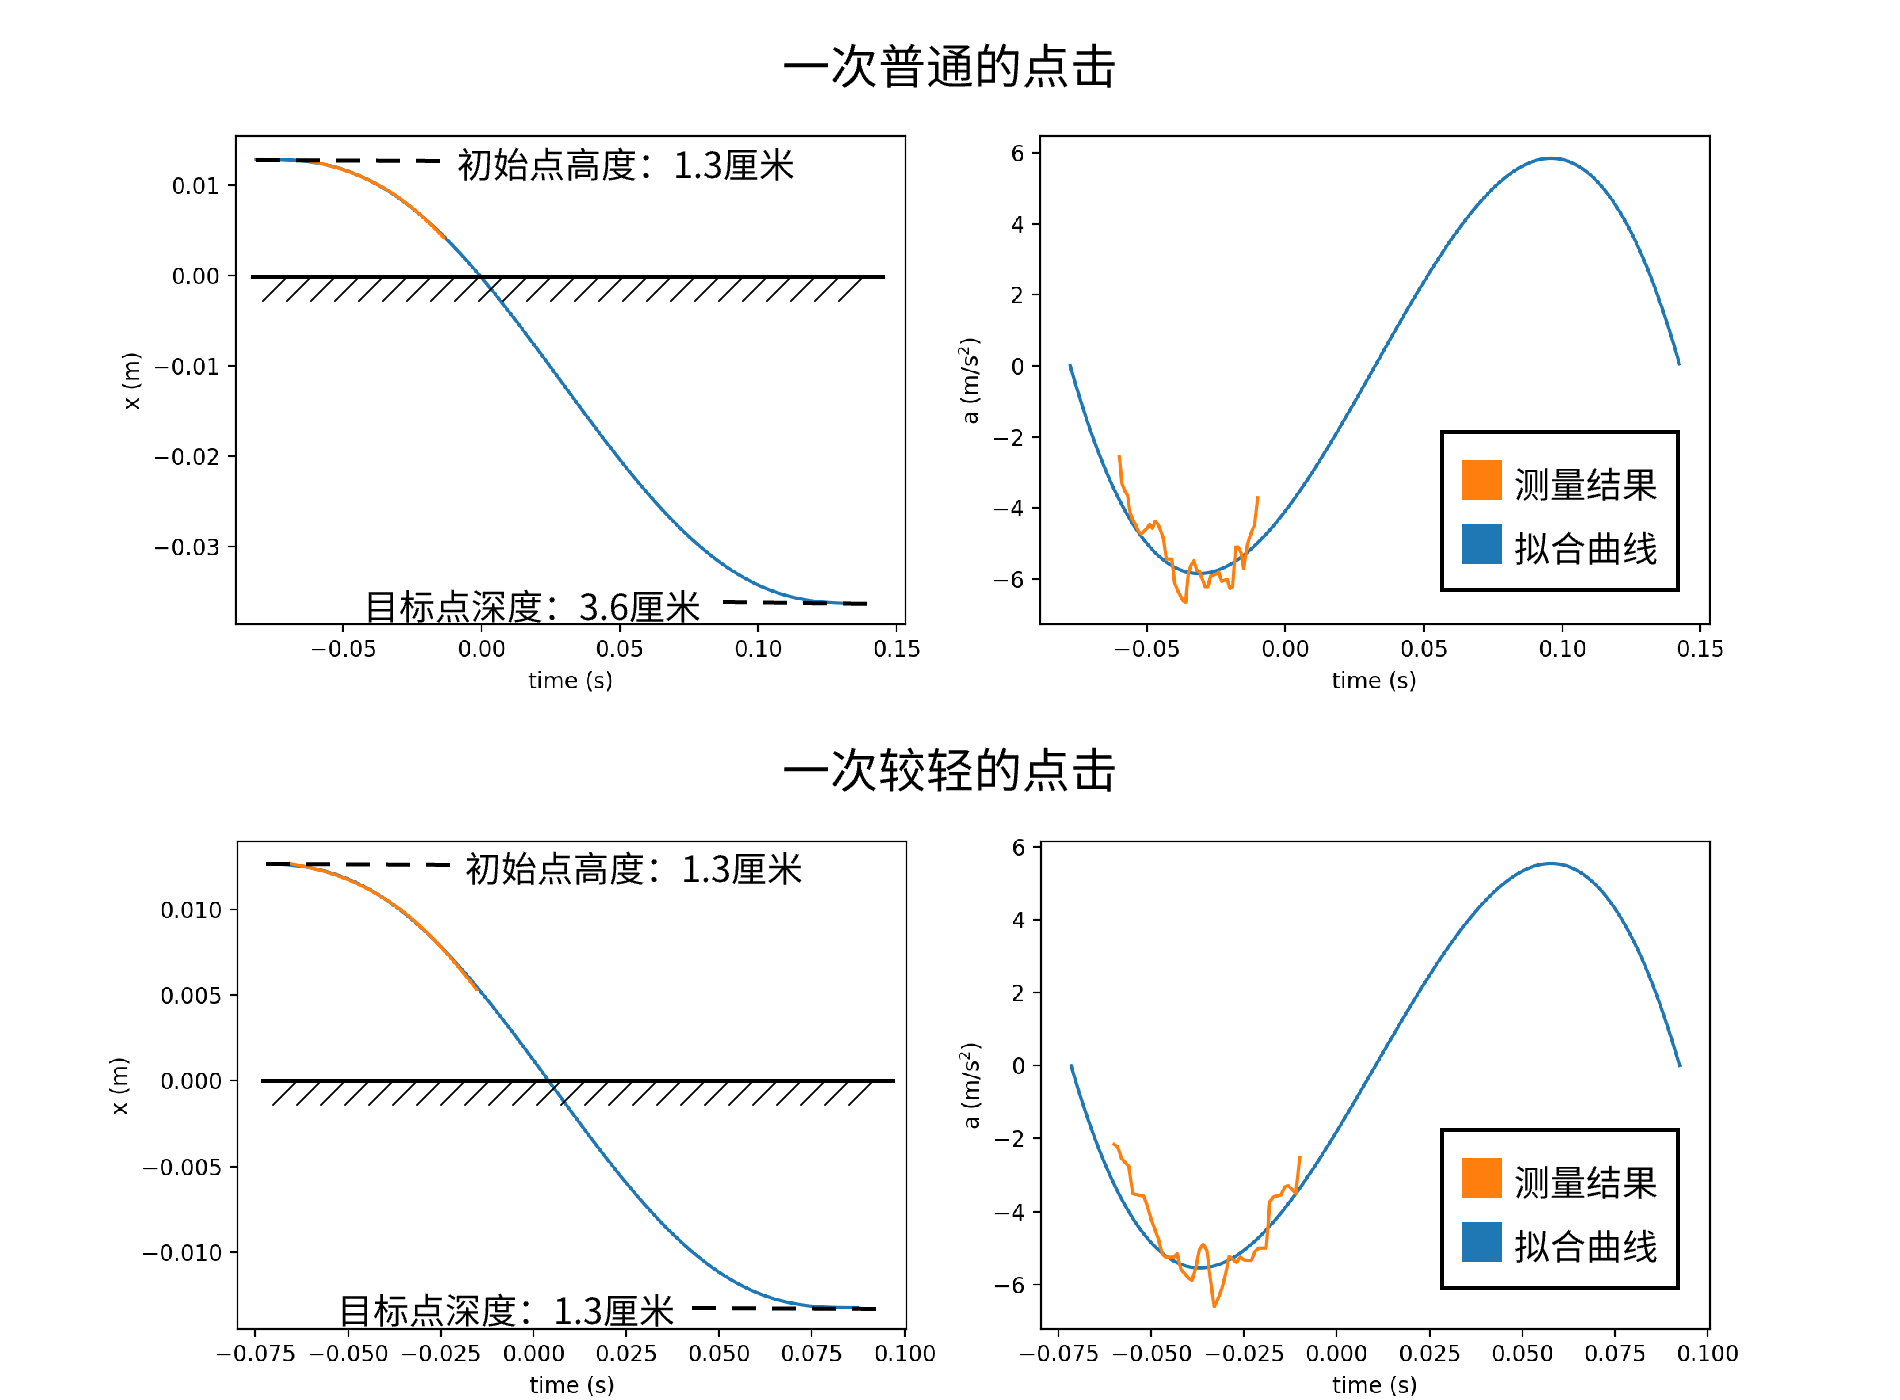
\includegraphics[width=0.8\linewidth]{model_fitting.png}
	\caption*{介绍}
	\caption{触摸运动计算模型的拟合实例}
	\label{fig:model_fitting}
\end{figure}

如上图所示是使用触摸运动计算模型拟合实际测量数据的两个实例,上方的两幅子图展示了一次普通力度点击的拟合效果,左上方是对触摸运动位移的拟合,右上方是对运动的加速度的拟合;下方的两幅子图展示了一次较轻点击的拟合效果。通过观察上图,读者很容易从中找到有用的信息,可用户指导触摸交互技术的改进。

\section{触摸运动的应用}

\textbf{(1)低延迟的触摸感知技术}:当实际测量结果与运动方程差异过大时,大到必定是外力作用(而不是手指运动或传感器误差时),可以判定为触摸事件的发生。

\textbf{(2)推测点击力度}:根据公式,可以精准计算触摸瞬间手指的速度,该速度与点击力度成正比。点击力度可用于拓展触摸交互的可达性[xx]。

\textbf{(3)为传感器的性能改进提供了指导}:例如,传感器的精度作用是平方级的,而传感器采样率的作用是线性的。

\textbf{(4)防误触技术}:在十指打字等连续触摸任务中,若对每只手指下落的过程拟合其运动方程,手指间运动方程的相关性是判断触摸意图的有力特征子。







\iffalse

其中,$\tau=\frac{t}{t_1-t_0}$表示当前时刻的运动进度。从公式中可以看出,无约束端到端运动在空间上沿直线运行,只在时间上存在一个先加速后减速的过程。

通过实验观察,我们发现了两种触摸运动,分别是:(1)长时触摸运动,即长按、拖拽等触摸过后手指保持与交互表面接触的触摸运动;(2)短时触摸运动,即轻敲、文本输入点击等触摸过后手指立即抬起的触摸运动。我们借鉴Tamar的手部运动模型[xx]来描述触摸运动,由于手部运动方程在笛卡尔坐标系的三个轴上的方程是独立的,且触摸运动的主要分量是手指与交互表面的距离$x$,以下我们仅研究$x$与时间$t$的关系:

\emph{“长时触摸运动:假设交互表面在触摸瞬间消失,长时触摸运动可描述为无约束端到端运动,其中起始点$x_0$是人产生触摸意图时手指的位置,手指将下落至位于交互表面之下的虚构目标点$x_1$,然后静止。”}

\emph{“短时触摸运动:假设交互表面在触摸瞬间消失,短时触摸运动可描述为过特定点的端到端运动,其中起始点$x_0$是人产生触摸意图时手指的位置,手指将下落至位于交互表面之下的虚构点$x_1$,随即抬起到目标点$x_2$。”}

【图:交互表面在触摸瞬间消失的情况】

对于无约束端到端运动,我们有$x^{'}(t_1)=0,x^{''}(t_1)=0$;对于上述过特定点的端到端运动,由于$x_1$是运动的最低点,手指下落经过$x_1$后立即上抬,因此手指在$x_1$点上的速度为零,且加速度大于零,即$x^{'}(t_1)=0,x^{''}(t_1)>0$。从公式可以看出,无论是长时触摸运动,还是短时触摸运动,其初始点$x_0$至虚构点$x_1$之间的运动方程都可以描述为:

\begin{equation}
	\begin{cases}
		x(t) \\
		s.t. x(0)=x_0,x^{'}(0)=x^{''}(0)=0,x(t_1)=x_1,x^{'}(t_1)=0,x^{''}(t_1)\geq0 \\
		min\frac{1}{2}\int_{0}^{t_1}\left(\frac{d^3x}{dt^3}\right)^2 dt
	\end{cases}
\end{equation}

但由于交互表面的存在,手指总是会在叨叨虚构点$x_1$之前被交互表面阻挡,瞬间停止,因此,只有起始点$x_0$到虚构点$x_1$之间

\subsection{过特定点的端到端运动}

与端到端的直线运动不同,现实生活中更多的手部运动沿弧线运行,根据Tamar的理论,现实生活中大部分弧线手部运动属于过特定点的端到端运动,即由下述用户意图引导的手部运动:

\emph{“在规定时间$t_2$内,最平稳地将手部从初始点$(x_0, y_0, z_0)$移动到目标点$(x_2, y_2, z_2)$,且必须在中途经过特定点$(x_1, y_1, z_1)$。”}

其中,“最平稳地”指的仍然是最小化手部运动急动度的平方的积分(公式\ref{equ:objective_function}),因此求解无约束端到端运动的方程等价于以下最优化问题:

\begin{equation}
	\begin{cases}
		x(t),y(t),z(t),t_1 \\
		s.t. x(0)=x_0,x^{'}(0)=x^{''}(0)=0,x(t_1)=x_1,x(t_2)=x_2,x^{'}(t_2)=x^{''}(t_2)=0 \\
		y(0)=y_0,y^{'}(0)=y^{''}(0)=0,y(t_1)=y_1,y(t_2)=y2,y^{'}(t_2)=y^{''}(t_2)=0 \\
		z(0)=x_0,z^{'}(0)=x^{''}(0)=0,z(t_1)=z_1,z(t_2)=z2,z^{'}(t_2)=z^{''}(t_2)=0 \\
		min\frac{1}{2}\int_{0}^{t_2}\left(\left(\frac{d^3x}{dt^3}\right)^2+\left(\frac{d^3y}{dt^3}\right)^2+\left(\frac{d^3z}{dt^3}\right)^2\right)dt
	\end{cases}
\end{equation}

上述最优化问题的解是:

\begin{equation}
	\begin{cases}
		x^{-}(\tau)=\frac{t_2^5}{720}(\pi_1(\tau_1^4(15\tau^4-30\tau^3)+\tau_1^3(80\tau^3-30\tau^4)-60\tau^3\tau_1^2+30\tau^4\tau_1-6\tau^5) \\ +c_1(15\tau^4-10\tau^3-6\tau^5))+x_0 \\
		x^{+}(\tau)=\frac{t_2^5}{720}(\pi_1(\tau_1^4(15\tau^4-30\tau^3+30\tau-15)+\tau_1^3(80\tau^3-30\tau^4-60\tau^2+10) \\ +c_1(15\tau^4-10\tau^3-6\tau^5+1))+x_2
	\end{cases}
\end{equation}

其中,$\tau=\frac{t}{t_2-t_0}$表示当前时刻的运动进度,$x^{-}(\tau)$是手部在经过特定点$(x_1, y_1, z_1)$之前(即$t<=t_1$)的运动方程,$x^{+}(\tau)$是手部在经过特定点$(x_1, y_1, z_1)$之后(即$t>t_1$)的运动方程。$t_1$的值可以通过动态优化问题[xx]求解。$\pi_1$和$c_1$是常数使得$x^{-}(\tau_1)=x^{+}(\tau_1)=x_1$。运动在y轴、z轴上的运动方程$y^{-}(\tau)$、$y^{+}(\tau)$、$z^{-}(\tau)$、$z^{+}(\tau)$与上述公式类似,且运动在三个轴上的方程相互独立。

\fi

